%Flo
\section{Introduction}
Several types of storage can be used in a computer system~:
\begin{itemize}
    \item \textbf{Primary storage} can be operated on directly by the CPU. It includes main memory and small cache memories. These data are \textit{volatile}.
    \item \textbf{Secondary storage} is used for online storage. Magnetic disks are more and more replaced by SSDs.
    \item \textbf{Tertiary storage} includes optical disks and tapes. Used for offline storage (archives, ...).
\end{itemize}
Data must always be copied into primary storage before it can be processed by the CPU. \\

A database stored on disk is organized as \textbf{files} of \textbf{records}. Generally a DB is too large to fit entirely in main memory, so there are strategies to copy parts of it into main memory during a program execution.



\section{Secondary Storage Devices}

Disk devices are \textbf{random access} secondary storage because any block may be accessed at random while magnetic tapes are \textbf{sequential access} devices because $n$ blocks must be scanned to read block number $n$.

\subsubsection*{Hard Disk Drive}

An HDD is composed of several \textbf{cylinders}, each containing \textbf{tracks} of the same size, each containing \textbf{sectors} that contain \textbf{blocks}. The hardware mechanism that reads or writes a block is the \textbf{head} that contains a mechanical arm to move around the disk. \\

\begin{samepage}

The time to transfer a disk block is given by $s + r + b$ where
\begin{itemize}
    \item $s$ is the \textbf{seek time} = time to position the head on the right track
    \item $r$ is the \textbf{rotational delay} = time for the block to rotate into position under the head. It depends on the \textbf{rpm} of the disk. So in average $r=\dfrac{1}{2} \times \dfrac{1}{60 \times rpm}$.
    \item $b$ is the \textbf{block transfer time}
\end{itemize}
\end{samepage}

Usually $s$ and $r$ are much more significant than $b$. That is why it is common to transfer several consecutive blocks. \\

\subsubsection*{Solid-state Drive}

An SSD is a set of interconnected flash memory cards. Any address is directly addressable so the data is less likely to be fragmented. It is faster because no mechanical delay but also more expensive.

\subsubsection*{Magnetic Tapes}
The data blocks of a magnetic tapes are accessed in \textbf{sequential order}. Tape access can then be slow so their main function is \textbf{backing up} the DB.



\section{Placing File Records on Disk}

A file is a sequence of records. It is made up of \textbf{fixed-length} or \textbf{variable-length} records. These records \textit{may} be of the same type.

\subsubsection*{Separating records}

For fixed-length records there is no need of separator. For variable-length records we can use a \textbf{separator} to place between records. Or one can give record lengths or offsets in block header. Also, in a file that includes records of different types, each record is preceded by a \textbf{record type} indicator.

\subsubsection*{Spanned records}

\begin{samepage}

Two main record organizations exist~:
\begin{itemize}
    \item \textbf{unspanned} : a record must be within one block. Much simpler but may waste space.
    \item \textbf{spanned} : a record can span over several blocks. Essential if record size > block size.
\end{itemize}
\end{samepage}

Figures~\ref{fig:chap16-unspanned} and~\ref{fig:chap16-spanned} show both strategies.

\begin{figure}[h]
    \centering
    \begin{subfigure}[b]{\linewidth}
        \centering
        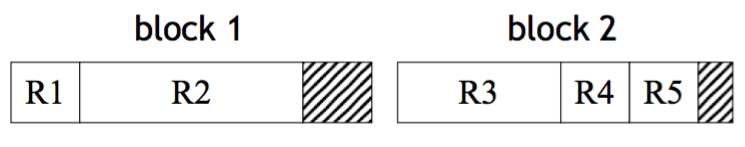
\includegraphics[scale=0.4]{chap16-unspanned.png}
        \caption{Unspanned}
        \label{fig:chap16-unspanned}
    \end{subfigure}
    
    \begin{subfigure}[b]{\linewidth}
        \centering
        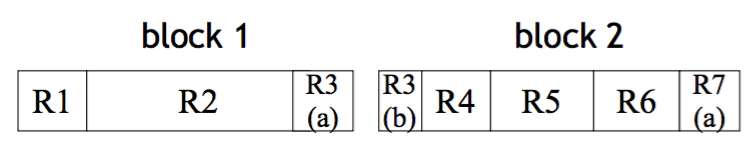
\includegraphics[scale=0.4]{chap16-spanned.png}
        \caption{Unspanned}
        \label{fig:chap16-spanned}
    \end{subfigure}
    \caption{Type of record organizations}
\end{figure}


\subsubsection*{Allocating File Blocks on Disk}
Two main techniques~:
\begin{itemize}
    \item \textbf{Contiguous allocation}~: file blocks are allocated to consecutive disk blocks. File expansion is hard but reading is very fast with double buffering.
    \item \textbf{Linked allocation}~: each file block contains a pointer to the next file block. Easy expand but slower reading.
\end{itemize}

Combinations of those two techniques are common such as \textbf{clustering} or \textbf{indexed allocation} or even combinations of these two.

\section{Operations on Files}
One access records in a file using a set of commands. Usually the program maintains a pointer to the current file record. The main commands are \textbf{open} and initialize a file, \textbf{find} a record matching a condition, \textbf{findnext} to iterate, \textbf{read} the file in a variable, \textbf{insert} a record, \textbf{delete} a record, \textbf{modify} a record, \textbf{close} the file, \textbf{reorganize} the file records, \textbf{read\_ordered} to read the records in a specific order.

\section{Various kinds of files}

\subsubsection*{Heap files}
Those are \textbf{unordered} files. Insertion is made at then end of the file and so is very efficient. But looking for a record is a \textit{linear search}.

\subsubsection*{Sorted files}
The records and the blocks in these files are \textbf{ordered} by some key value. Looking for a record is a \textit{binary search} but \textbf{only} if we access a record based on the key value. For other values it is a linear search. Record insertion and deletion are expensive because the records must remain ordered.

\subsubsection*{Hash files}
The search condition is an equality condition on a single field~: the \textbf{hash field}. The \textbf{hash function} is applied to the hash field value of a record $r$ and yields the address of the disk block in which $r$ is stored. Two main techniques exist~:

\begin{itemize}
    \item \textbf{Internal hashing} is implemented with a \textbf{hash table} and an array of records of length $M$. Then we have $M$ different values that the hash function can return.
    \item \textbf{External hashing} is implemented with \textbf{buckets}, each of which holds multiple records. The hashing function maps a key into a relative bucket.
\end{itemize}

In both cases \textbf{collision} may happen. It is less severe in external hashing because several records may fit in one bucket.